\section{Main Experiment}
This section describes the experimental setup and evaluation results. We assess our approach on two benchmarks: OpenAGI \citep{ge2024openagi} which focuses on complex decision-making tasks that require reasoning over both vision and language modalities including 312 multi-step tasks, and TravelPlanner \citep{xie2024travelplanner} which targets travel planning scenarios with 180 tasks. We evaluate the performance of our dynamic speculative planning framework and compare it to a set of baselines.

% \textbf{Benchmarks}
% OpenAGI focuses on complex decision-making tasks that require reasoning over both vision and language modalities. Tasks involve composing these tools in a sequential order to solve high-level goals. This benchmark provides 312 multi-step tasks. TravelPlanner targets diverse and realistic tasks, especially travel planning scenarios. Agents must generate comprehensive and sequential plans that address transportation, daily meals, and accommodation, while adhering to multiple restrictions. We use its validation dataset as one of our benchmark which provides 180 multi-step tasks.

\textbf{The speculative step predictor} uses DistilBERT for its efficiency and expressive capacity in forecasting the speculation step $k$ from a given state. The model is fine-tuned using expectile regression to learn the bias and adaptively adjust its predictions based on the collected data. The model is optimized using AdamW with a learning rate of $1\times10^{-5}$, batch size $16$. Each training process iterates over $3$ epochs on a randomly sampled replay buffer (size $2,\!500$). For multi-step return estimation, we adopt $\lambda$-return blending ($\lambda=0.95$) to balance bias-variance trade-offs during reward propagation. 
% This configuration ensures stable adaptation to dynamic interaction patterns while maintaining real-time responsiveness during speculative execution.

\textbf{LLM backbones for agents} from the GPT and DeepSeek families are used in DSP. Below are their cost profiles:
%across different model architectures and cost profiles.
(1) \emph{GPT-4.1-mini} costs \$0.40/\$1.60 (prompt/generation per million tokens).
(2) \emph{DeepSeek}: We use DeepSeek-chat as $\approxi$'s backbone and DeepSeek-reasoner as $\target$'s backbone, with respective costs of \$0.27/\$1.10 and \$0.55/\$2.19.

\textbf{Baselines} are chosen to be speculative planning with fixed $k$, which is chosen independently of the environment’s characteristics or the task requirements.
We evaluate three configurations for the baseline with $k\in\{2, 4, 6\}$ which are incrementally more aggressive in efficiency.
%: (1) \( k = 2 \): A low step value that prioritizes a more conservative approach, focusing on cost reduction. (2) \( k = 4 \): A moderate step value balancing cost and efficiency. (3) \( k = 6 \): The largest feasible step, which approximates the most optimal time-saving performance. The fixed \( k \) baselines represent the traditional approach to speculative planning, where \( k \) is predefined and does not adapt to the changing requirements of the task.

%\subsection{Experimental Settings}
\textbf{Four DSP configurations} are utilized for experiments: (1) \emph{Direct-Generation}: $\approxi$ generates the action directly for each step in a single LLM call, without any intermediate reasoning. (2) \emph{Chain-of-Thought (CoT)}: $\approxi$ first reasons about the current step and then generates the action based on the reasoning, all within a single LLM call. (3) \emph{ReAct}: $\target$ first deliberates on the action to take, then generates the action through two distinct LLM calls. (4) \emph{Multi-agent Debate (MAD)}: two target agents debate in two rounds, with each agent proposing and refining actions.%, with five LLM calls in total.

% \textbf{Backbone Models for Agent}  Models from the GPT and DeepSeek families are evaluated to demonstrate the generality of DSP across different model architectures and cost profiles.
% (1) \emph{GPT-4.1-mini} costs \$0.40/\$1.60 (prompt/generation per million tokens).
% (2) \emph{DeepSeek}: We employ DeepSeek-chat as $\approxi$'s backbone and DeepSeek-reasoner as $\target$'s backbone, with respective costs of \$0.27/\$1.10 and \$0.55/\$2.19. 



\subsection{Evaluation Metrics}
Evaluation metrics are designed along three critical dimensions to assess speculative planning (SP) systems: \emph{latency reduction}, \emph{resource overhead}, and \emph{concurrency dynamics}. This triad captures the trade-offs in real-world deployment, where effective systems must accelerate task completion while respecting resource constraints and API concurrency limits.
% All metrics are computed per planning step and averaged over the task sequence to reduce variance and bias arising from stochasticity in the number of target steps, as longer target steps tend to incur greater time and token consumption. This normalization ensures fair comparison and yields a more robust estimate of overall performance. 
% For \emph{latency reduction} and \emph{resource overhead}, we adopt fixed $k=2$ as the baseline configuration for evaluating various speculation strategies, as it represents the minimal non-trivial setting that offers meaningful acceleration with minimal resource cost: on the OpenAGI benchmark, the fixed $k=2$ configuration typically provides 15\%-25\% time reduction compared to sequential planning. Efficiency and economy metrics are reported as ratios relative to the fixed $k=2$ baseline. $\text{T}(\times)$, $\text{P}(\times)$, $\text{G}(\times)$, and $\text{Cost}(\times)$ represent relative latency, prompt token usage, generation token usage, and monetary cost, respectively. $\overline{MC}$ denotes average peak concurrency (maximum parallel LLM calls), and $\overline{K}$ is the average predicted step length per episode. 

Efficiency and economy metrics are reported through two complementary perspectives:

\textbf{Relative change metrics ($\Delta$)} quantify performance against sequential execution, capturing \textit{net improvements or overheads} introduced by speculative planning.
\textbf{Absolute ratio metrics ($\times$)} measure resource consumption relative to the fixed $k=2$ baseline, enabling \textit{cross-strategy comparison} for practical deployment decisions.

The fixed $k=2$ baseline is adopted as it represents the minimal non-trivial setting that offers meaningful acceleration with minimal resource cost. As empirically validated on the OpenAGI benchmark, this configuration typically provides 15\%-25\% latency reduction ($\Delta \text{T}$) compared to sequential planning while maintaining low token overhead. This makes it an ideal reference point for comparing more advanced speculation strategies. Specifically:

$\text{T}(\times)$, $\text{P}(\times)$, $\text{G}(\times)$, and $\text{Cost}(\times)$ denote absolute ratios of latency, prompt tokens, generation tokens, and monetary cost versus the $k=2$ baseline.
$\Delta \text{T}$, $\Delta \text{P}$, $\Delta \text{G}$, and $\Delta \text{Cost}$ represent relative percentage changes versus sequential planning.
$\overline{MC}$ denotes average peak concurrency (maximum parallel LLM calls), and $\overline{K}$ is the average predicted step length per episode.

\paragraph{1. Time Decrease ($\Delta {\text{T}}$)} 
Quantifies the relative latency reduction when using speculative planning. 
Specifically, for each task, we calculate the total time taken to complete the task under SP ($T^{\text{SP}}$) and sequential planning ($T^{\text{seq}}$). The percentage time saving is then calculated as:
\[
\Delta {\text{Time}} = \frac{1}{N} \sum_{i=1}^N \left(1 - \frac{T^{\text{SP}}_i}{T^{\text{seq}}_i}\right) \times 100\%
\]
where $N$ is the total number of tasks. Positive values indicate time savings.

\paragraph{2. Cost and Token Increase}
% In our experiments, we evaluate both \emph{token increase} and \emph{monetary cost increase} to provide a comprehensive understanding of the additional resources consumed due to speculative planning. The motivation for considering both metrics stems from the varying costs associated with different large language models (LLMs) and APIs. \emph{Token increase} serves as a general metric for resource consumption, while \emph{cost increase} can offer a more tangible and comparable view of the cost implications.

Token increase captures the \emph{redundant} resources consumed by speculative planning as a result of incorrect speculation. While the primary goal of speculative planning is to reduce latency and enhance efficiency, it still incurs a minimum cost. Even with perfect accuracy in speculative planning (\emph{i.e.}, the approximation agent makes correct predictions for every step), the cost must at least include the \emph{baseline cost} — the minimal overhead associated with sequential planning of both the target and approximation agents. Thus, we define the baseline for token increase as the sum of the planning costs for the target agent and approximation agent operating sequentially, which represents the least amount of resources required for completing the task with speculation. Any increase in token usage beyond this baseline reflects the additional overhead introduced by speculative failures, capturing the waste generated from incorrect predictions by the approximation agent.

% To isolate the overhead from speculative failures, we measure \emph{token increase} relative to the \textbf{minimal required cost}—defined as the token consumption of both target and approximation agents with perfect accuracy in speculative planning (i.e., the approximation agent makes correct predictions for every step). This baseline represents the intrinsic cost of SP.

Since the cost per token can differ for \emph{prompt tokens} and \emph{generation tokens}, we separately evaluate these components and also provide a combined metric for \emph{total cost increase}.

\textbf{Prompt Token Increase ($\Delta P$)} This measures the increase in prompt tokens due to redundant prompt usage in SP. Let $p^{\text{seq}}_i = p^{\text{target}}_i + p^{\text{approx}}_i$ be the baseline prompt tokens (the sum of target and approximation prompts under sequential execution), and $p^{\text{SP}}_i$ be the prompt tokens used under SP (parallel execution). The prompt token increase is calculated as:
\begin{equation}
    \Delta P = \frac{1}{N} \sum_{i=1}^N \left(\frac{p^{\text{SP}}_i}{p^{\text{seq}}_i} - 1\right) \times 100\%
\end{equation}
    
\textbf{Generation Token Increase ($\Delta G$)} This metric captures the increase in generation tokens caused by incorrect speculation. Let $g^{\text{seq}}_i = g^{\text{target}}_i + g^{\text{approx}}_i$ represent the baseline generation tokens (the sum of target and approximation generations under sequential execution), and $g^{\text{SP}}_i$ the generation tokens used under SP. The generation token increase is calculated as:
\begin{equation}
    \Delta G = \frac{1}{N} \sum_{i=1}^N \left(\frac{g^{\text{SP}}_i}{g^{\text{seq}}_i} - 1\right) \times 100\%
\end{equation}


\textbf{Total Cost Increase ($\Delta {\text{Cost}}$)} This metric quantifies the relative increase in cost between speculative planning (SP) and sequential planning (seq) strategies. Specifically, we define the total cost increase as:
\begin{equation}
    \Delta \text{Cost} = \frac{1}{N} \sum_{i=1}^N
    \left( \frac{PC^{\text{SP}}_i + GC^{\text{SP}}_i}{PC^{\text{seq}}_i + GC^{\text{seq}}_i} - 1 \right) \times 100\%
\end{equation}

where $PC^{\text{SP}}_i$ and $PC^{\text{seq}}_i$ represent the prompt costs of task $i$ for SP and sequential strategies, and $GC^{\text{SP}}_i$ and $GC^{\text{seq}}_i$ represent the corresponding generation costs. These costs are computed as follows:

\begin{equation}
    PC^{\text{SP}}_i = ap^{\text{SP}}_i \cdot \text{cost}_{\text{ap}} + tp^{\text{SP}}_i \cdot \text{cost}_{\text{tp}}
\end{equation}

\begin{equation}
    PC^{\text{seq}}_i = ap^{\text{seq}}_i \cdot \text{cost}_{\text{ap}} + tp^{\text{seq}}_i \cdot \text{cost}_{\text{tp}}
\end{equation}

\begin{equation}
    GC^{\text{SP}}_i = ag^{\text{SP}}_i \cdot \text{cost}_{\text{ag}} + tg^{\text{SP}}_i \cdot \text{cost}_{\text{tg}}
\end{equation}

\begin{equation}
    GC^{\text{seq}}_i = ag^{\text{seq}}_i \cdot \text{cost}_{\text{ag}} + tg^{\text{seq}}_i \cdot \text{cost}_{\text{tg}}
\end{equation}

Here, $ap^{\text{SP}}_i$ and $tp^{\text{SP}}_i$ represent the number of prompt tokens for the approximation and target in the SP strategy at task $i$, and $ap^{\text{seq}}_i$ and $tp^{\text{seq}}_i$ represent the number of prompt tokens for the approximation and target in the sequential planning at task $i$. Similarly, $ag^{\text{SP}}_i$, $tg^{\text{SP}}_i$, $ag^{\text{seq}}_i$ and $tg^{\text{seq}}_i$ represent the corresponding number of generation tokens. For cost, $\text{cost}_{\text{ap}}$ and $\text{cost}_{\text{tp}}$ are the costs for the approximation and target API for prompt tokens, while $\text{cost}_{\text{ag}}$ and $\text{cost}_{\text{tg}}$ are the corresponding costs for generation tokens.

By computing the total cost increase, we can quantify the trade-off between speculative planning and sequential planning in terms of the associated computational costs, helping to assess the efficiency of the proposed approach.

\paragraph{3. Absolute Time Ratio (T($\times$))} This metric quantifies the ratio of the absolute time in the current configuration compared to the baseline configuration (fix $k=2$), as it represents the minimal non-trivial setting that offers meaningful acceleration with minimal resource cost. It is calculated as:
\[
\text{T}(\times) = \frac{T^{\text{current}}}{T^{\text{k=2}}}
\]

\paragraph{4. Absolute Cost and Token Ratio}
This metric measures the ratio of the absolute token usage and cost in the current configuration compared to the baseline configuration (fix $k=2$).

\textbf{Absolute Prompt Token Ratio (P($\times$))}
\[
\text{P}(\times) = \frac{p^{\text{current}}_i}{p^{\text{k=2}}_i}
\]

\textbf{Absolute Generation Token Ratio (G($\times$))} 
\[
\text{G}(\times) = \frac{g^{\text{current}}_i}{g^{\text{k=2}}_i}
\]

\textbf{Absolute Cost Ratio (Cost($\times$))}
\[
\text{Cost}(\times) = \frac{C^{\text{current}}}{C^{\text{k=2}}}
\]

\paragraph{5. Concurrency Dynamics}
Evaluating the concurrency behavior of speculative planning (SP) is essential for understanding its real-world deployability. Modern systems often impose limits on simultaneous API requests due to infrastructure constraints or cost-efficiency considerations. Excessive concurrency can lead to API throttling, degraded performance, or instability, making it critical to monitor and control parallel request patterns. To quantify this behavior, we introduce two metrics.

\textbf{Average Max Concurrent API Calls ($\overline{MC}$)} For each task $i$, $MC_i$ denotes the peak number of overlapping API requests during speculative execution. $\overline{MC}$ is calculated as:
\begin{equation}
\overline{MC} = \frac{1}{N} \sum_{i=1}^N {MC}_i
\end{equation}
where $N$ is the number of tasks. This metric reflects how aggressively a system exploits parallelism and whether it respects concurrency constraints under varying speculative policies.

\textbf{Average Speculative Step ($\overline{K}$)} In addition to peak concurrency ($\overline{MC}$), which captures brief spikes of load, we aim to characterize the \emph{average} concurrency of the planning process over the planning process, as it correlates with sustained system pressure. However, the instantaneous concurrency varies continuously over time. Precisely computing the time-averaged number of concurrent API calls would require fine-grained logs of every call’s start and end time, which is often impractical. To address this, we use the average speculative step $\overline{K}$ as a proxy for the true average concurrency. Let $M$ be the total number of planning episodes, and $k_i$ be the speculative steps used in episode $i$. We define
\begin{equation}
\overline{K} = \frac{1}{M} \sum_{i=1}^M {k}_i
\end{equation}
Because each target-agent computation is relatively long-running, the $k_i$ speculative calls in episode $i$ tend to overlap in time. In practice, this means the average concurrency during episode $i$ is effectively $k_i$. Averaging these values over all episodes therefore yields a meaningful estimate of the sustained concurrency.



\subsection{Main Experiment Result}

% \begin{minipage}{\textwidth}
\begin{table}[hbtp]
    \captionsetup{skip=2pt}
    \caption{Dynamic $k$ vs. Fixed $k$ Strategies on \textbf{OpenAGI} benchmark with \textbf{GPT} backbone}
    \label{tab:main_s12}
    \centering
    \resizebox{\textwidth}{!}{
    \begin{tabular}{lrrrrrrrrrrrr}
        \toprule
          \multirow{3}{*}{\bf Mode} & \multicolumn{6}{c}{\bf Direct-ReAct (Setting 1)} & \multicolumn{6}{c}{\bf CoT-MAD (Setting 2)} \\
          \cmidrule(lr){2-7} \cmidrule(lr){8-13} 
          & $\text {T ($\times$)}$ & $\text {P ($\times$)}$ & $\text {G ($\times$)}$ & $\text {Cost ($\times$)}$ & $\overline{MC}$ & $\overline{K}$ & $\text {T ($\times$)}$ & $\text {P ($\times$)}$ & $\text {G ($\times$)}$ & $\text {Cost ($\times$)}$ & $\overline{MC}$ & $\overline{K}$ \\
          \midrule 
            Fix (k = 2) & 1.00 & 1.00 & 1.00 & 1.00 & 3.00 & 2.00 & 1.00 & 1.00 & 1.00 & 1.00 & 3.00 & 2.00\\
            Fix (k = 4) & 0.92 & 1.56 & 1.23 & 1.41 & 4.95 & 4.00 & 0.83 & 1.41 & 1.38 & 1.37 & 4.97 & 4.00\\
            Fix (k = 6) & \textbf{0.90} & 2.24 & 1.57 & 1.92 & 6.32 & 6.00 & 0.81 & 1.87 & 1.75 & 1.77 & 6.44 & 6.00\\
            \hdashline
           \hdashline
            Dyn. ($\tau$=0.5) & 1.01 & 0.87 & 0.91 & \textbf{0.88} & 4.33 & 1.78 & 0.98 & 0.95 & 0.95 & \textbf{0.95} & 4.44 & 2.10\\
            Dyn. ($\tau$=0.8) & 0.97 & 0.97 & 0.98 & 0.97 & 4.41 & 2.33 & 0.89 & 1.04 & 1.04 & 1.04 & 4.73 & 2.67\\
            Dyn. ($\tau$=0.9) & 0.95 & 1.04 & 1.00 & 1.02 & 4.56 & 2.47 & 0.86 & 1.12 & 1.11 & 1.11 & 5.22 & 3.03\\
            Dyn. ($\tau$=0.95) & 0.94 & 1.12 & 1.07 & 1.09 & 4.75 & 2.88 & 0.85 & 1.26 & 1.25 & 1.24 & 5.64 & 3.58\\
            Dyn. ($\tau$=0.99) & 0.91 & 1.32 & 1.19 & 1.25 & 5.24 & 3.59 & 0.82 & 1.41 & 1.37 & 1.37 & 5.87 & 4.06\\
            \hdashline
            Dyn. (offset=1) & 0.92 & 1.10 & 1.06 & 1.08 & 4.86 & 2.75 & 0.88 & 1.11 & 1.09 & 1.10 & 4.95 & 2.80\\
            Dyn. (offset=2) & \textbf{0.90} & 1.33 & 1.15 & 1.25 & 5.13 & 3.47 & \textbf{0.80} & 1.29 & 1.27 & 1.27 & 5.60 & 3.99\\
            \bottomrule
        \end{tabular}
    }
\end{table}

\begin{table}[hbtp]
    \caption{Dynamic $k$ vs. Fixed $k$ Strategies on \textbf{OpenAGI} benchmark with \textbf{DeepSeek} backbone}
    \captionsetup{skip=2pt}
    \label{tab:main_s34}
    \centering
    \resizebox{\textwidth}{!}{
    \begin{tabular}{lrrrrrrrrrrrr}
        \toprule
          \multirow{3}{*}{\bf Mode} & \multicolumn{6}{c}{\bf Direct-ReAct (Setting 3)} & \multicolumn{6}{c}{\bf CoT-MAD (Setting 4)} \\
          \cmidrule(lr){2-7} \cmidrule(lr){8-13} 
          & $\text {T ($\times$)}$ & $\text {P ($\times$)}$ & $\text {G ($\times$)}$ & $\text {Cost ($\times$)}$ & $\overline{MC}$ & $\overline{K}$ & $\text {T ($\times$)}$ & $\text {P ($\times$)}$ & $\text {G ($\times$)}$ & $\text {Cost ($\times$)}$ & $\overline{MC}$ & $\overline{K}$ \\
          \midrule 
            Fix (k = 2) & 1.00 & 1.00 & 1.00 & 1.00 & 3.00 & 2.00 & 1.00 & 1.00 & 1.00 & 1.00 & 3.00 & 2.00 \\
            Fix (k = 4) & 0.89 & 1.58 & 1.50 & 1.55 & 4.92 & 4.00 & 0.89 & 1.51 & 1.47 & 1.49 & 4.94 & 4.00\\
            Fix (k = 6) & \textbf{0.87} & 2.04 & 1.86 & 1.98 & 6.33 & 6.00 & \textbf{0.87} & 1.86 & 1.80 & 1.83 & 6.59 & 6.00\\
             \hdashline
           \hdashline
            Dyn. ($\tau$=0.5) & 1.04 & 0.93 & 0.94 & \textbf{0.93} & 3.89 & 1.69 & 1.07 & 0.94 & 0.94 & \textbf{0.94} & 3.78 & 1.54\\
            Dyn. ($\tau$=0.8) & 0.98 & 1.02 & 1.02 & 1.02 & 4.20 & 2.08 & 0.97 & 1.08 & 1.08 & 1.08 & 4.57 & 2.31\\
            Dyn. ($\tau$=0.9) & 0.95 & 1.12 & 1.12 & 1.12 & 4.45 & 2.58 & 0.93 & 1.16 & 1.15 & 1.16 & 4.69 & 2.65\\
            Dyn. ($\tau$=0.95) & 0.92 & 1.17 & 1.19 & 1.18 & 4.78 & 2.83 & 0.90 & 1.24 & 1.22 & 1.23 & 5.12 & 3.12\\
            Dyn. ($\tau$=0.99) & 0.88 & 1.42 & 1.40 & 1.41 & 5.46 & 3.85 & 0.88 & 1.39 & 1.36 & 1.38 & 5.29 & 3.75\\
             \hdashline
            Dyn. (offset=1) & 0.93 & 1.11 & 1.12 & 1.11 & 4.39 & 2.58 & 0.91 & 1.15 & 1.15 & 1.15 & 4.48 & 2.80\\
            Dyn. (offset=2) & \textbf{0.87} & 1.35 & 1.34 & 1.34 & 4.99 & 3.53 & 0.88 & 1.36 & 1.33 & 1.35 & 5.38 & 3.85\\
           \bottomrule
    \end{tabular}
    }
\end{table}

\begin{table}[hbtp]
    \captionsetup{skip=2pt}
    \caption{Dynamic $k$ vs. Fixed $k$ Strategies on \textbf{Travel Planner} benchmark with \textbf{GPT} backbone}
    \label{tab:tp_main_res}
    \centering
    \resizebox{\textwidth}{!}{
    \begin{tabular}{lrrrrrrrrrrrr}
        \toprule
          \multirow{3}{*}{\bf Mode} & \multicolumn{6}{c}{\bf Direct-ReAct (Setting 1)} & \multicolumn{6}{c}{\bf CoT-MAD (Setting 2)} \\
          \cmidrule(lr){2-7} \cmidrule(lr){8-13} 
          & $\text {T ($\times$)}$ & $\text {P ($\times$)}$ & $\text {G ($\times$)}$ & $\text {Cost ($\times$)}$ & $\overline{MC}$ & $\overline{K}$ & $\text {T ($\times$)}$ & $\text {P ($\times$)}$ & $\text {G ($\times$)}$ & $\text {Cost ($\times$)}$ & $\overline{MC}$ & $\overline{K}$ \\
          \midrule 
            Fix (k = 2) & 1.00 & 1.00 & 1.00 & 1.00 & 3.00 & 2.00 & 1.00 & 1.00 & 1.00 & 1.00 & 3.00 & 2.00\\
            Fix (k = 4) & 0.89 & 1.95 & 1.39 & 1.95 & 5.00 & 4.00 & \textbf{0.96} & 1.48 & 1.22 & 1.46 & 4.62 & 4.00\\
            Fix (k = 6) & \textbf{0.87} & 2.86 & 1.67 & 2.91 & 6.99 & 6.00 & 0.97 & 1.67 & 1.25 & 1.64 & 5.37 & 6.00\\
            \hdashline
           \hdashline
            Dyn. ($\tau$=0.5) & 1.05 & 0.81 & 0.92 & \textbf{0.80} & 4.28 & 1.46 & 1.05 & 0.85 & 0.88 & \textbf{0.84} & 4.09 & 1.30\\
            Dyn. ($\tau$=0.8) & 0.99 & 0.95 & 0.97 & 0.93 & 4.60 & 1.88 & 1.05 & 0.86 & 0.89 & 0.85 & 4.00 & 1.42\\
            Dyn. ($\tau$=0.9) & 0.95 & 1.06 & 1.03 & 1.04 & 4.96 & 2.21 & 1.01 & 0.99 & 0.96 & 0.98 & 4.03 & 1.79\\
            Dyn. ($\tau$=0.95) & 0.93 & 1.20 & 1.09 & 1.18 & 5.19 & 2.55 & 0.98 & 1.02 & 0.97 & 1.01 & 4.00 & 2.10\\
            Dyn. ($\tau$=0.99) & 0.92 & 1.49 & 1.20 & 1.48 & 5.32 & 3.10 & \textbf{0.96} & 1.25 & 1.13 & 1.24 & 4.58 & 2.94\\
            \hdashline
            Dyn. (offset=1) & 1.03 & 0.96 & 0.97 & 0.94 & 4.31 & 2.30 & 0.99 & 1.05 & 1.01 & 1.04 & 4.08 & 2.16\\
            Dyn. (offset=2) & 0.99 & 1.16 & 1.04 & 1.12 & 4.91 & 3.22 & 0.98 & 1.33 & 1.16 & 1.32 & 4.33 & 2.98\\
            \bottomrule
        \end{tabular}
    }
\end{table}
% \end{minipage}

\begin{figure}[htbp]
\centering
\captionsetup{skip=1pt}
\subcaptionbox{Prompt Token Increase vs Time Decrease}
{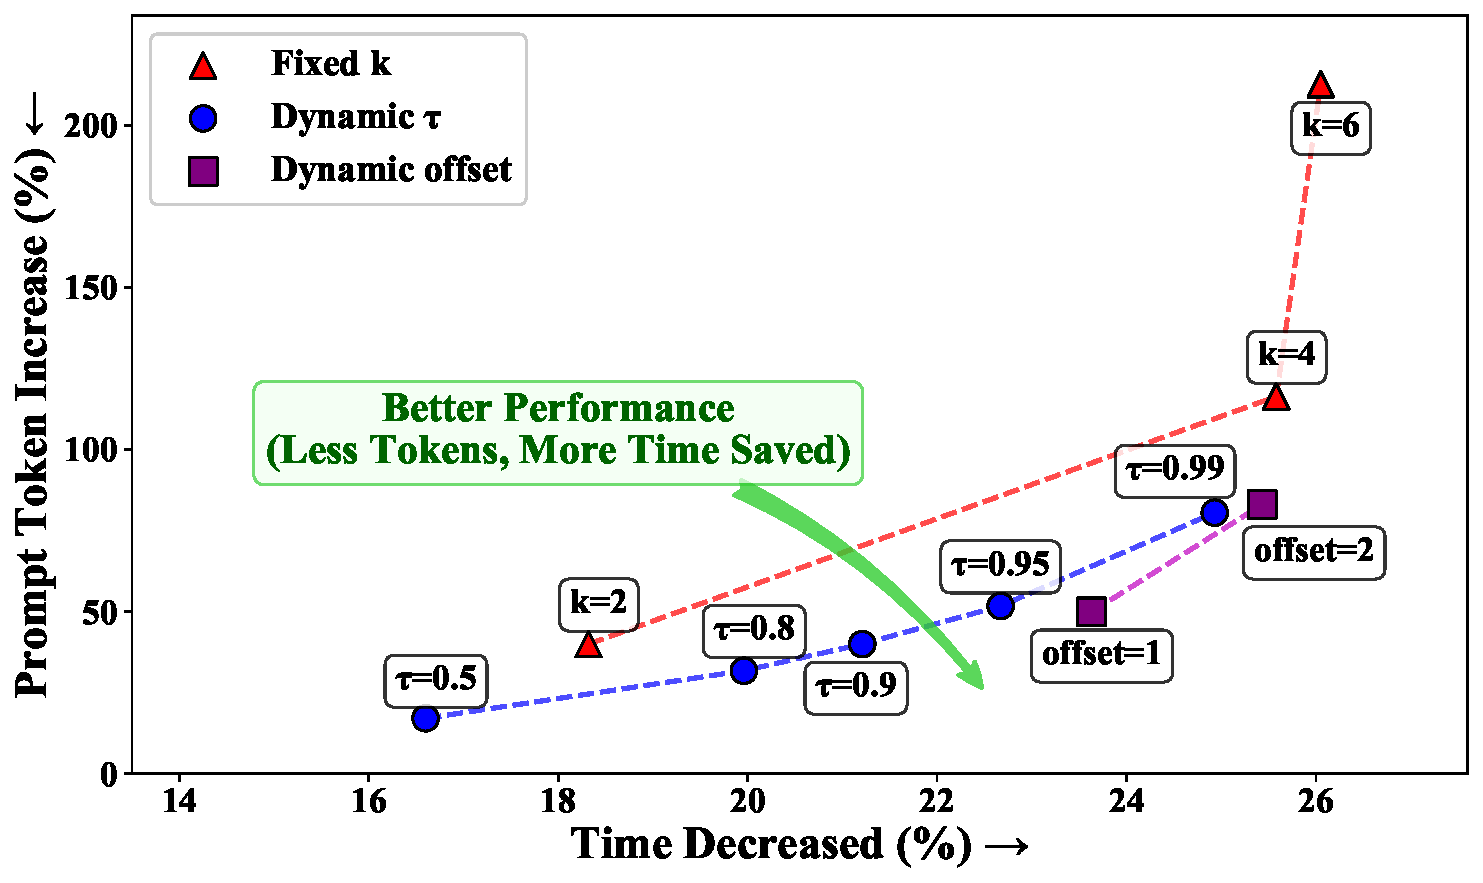
\includegraphics[width=0.44\textwidth]{fig/openagi_react_prompt_vs_time.pdf}}
\hfill
\subcaptionbox{Generation Token Increase vs Time Decrease}
{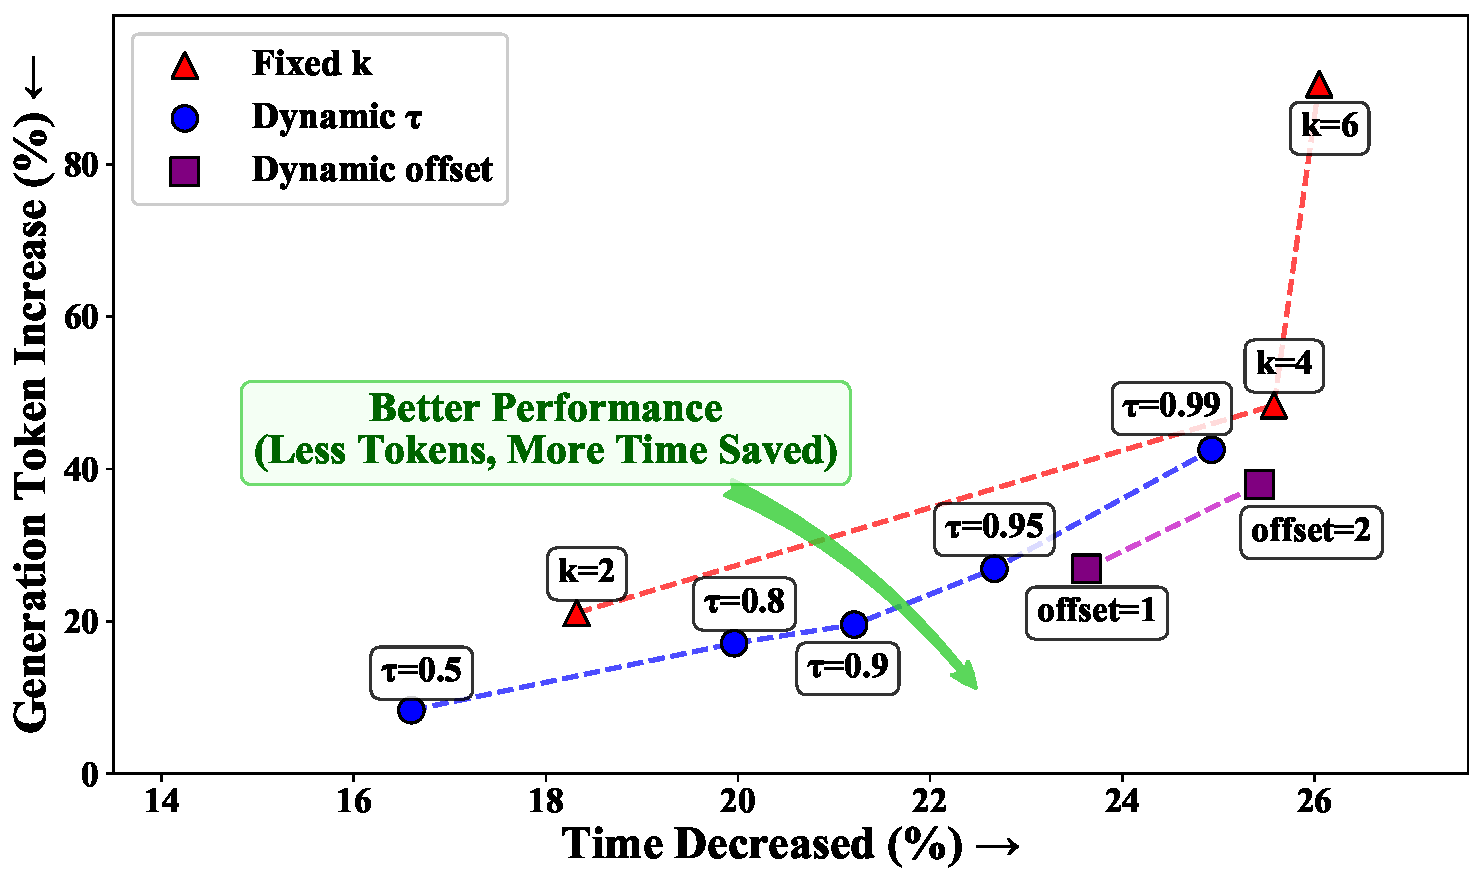
\includegraphics[width=0.44\textwidth]{fig/openagi_react_gen_vs_time.pdf}}
\captionsetup{skip=-1pt}
\caption{Performance trade-off between acceleration and token increase between Fix-$k$, Dynamic-$\tau$ and Dynamic-offset SP. (a) Prompt token and (b) Generation token increase vs. latency reduction, both relative to a normal-plan baseline. 
% Detailed metric definitions and corresponding performance analysis are provided in \cref{appendix:eval_metrics} and \cref{appendix:actual_performance}.
% Red dashed lines with triangle markers indicate the fixed-$k$ baseline, and blue dashed lines with circle markers indicate the dynamic-$\tau$ method. Each data point is labeled with its corresponding $k$ or $\tau$ value. The green arrow denotes the direction of better performance.
}
\label{fig:scatter_openagi}
\end{figure}

As shown in \cref{tab:main_s12}, \cref{tab:main_s34}, \cref{tab:tp_main_res}, and \cref{fig:scatter_openagi}, our experiments validate that DSP achieves superior Pareto efficiency compared to fixed-k baselines. Key findings include:

\subsubsection{Cost-Efficiency Dominance}

DSP demonstrates \textbf{strict Pareto dominance} through two operational modes:

\textbf{(1) Equivalent Latency, Lower Cost} \emph{On the OpenAGI benchmark}: 
In \textbf{setting 1}, Dyn. ($\tau=0.99$) and Dyn. ($\text{offset}=2$) achieves comparable time reduction to Fix ($k=6$) with a \textbf{34.9\%} (1.25$\times$ compared with 1.92$\times$ as in \cref{tab:main_s12}) reduction in cost. 
Dyn. ($\text{offset}=1$) saved \textbf{23.4\%} total cost compared to Fix ($k=4$) with comparable latency reduction.
Compared to Fix ($k=2$), Dyn. ($\tau=0.5$) achieves a similar latency reduction and a substantial 12\% decrease in token cost. 
In \textbf{setting 2}: Dyn. ($\tau=0.95$) achieves comparable latency reduction to Fix ($k=4$) while saving 9.49\% cost. Dyn. ($\text{offset}=2$) yields a marginally better acceleration than Fix ($k=6$), and significantly reduces token cost by $\textbf{28.25\%}$.
In \textbf{setting 3}: % Dyn. ($\tau=0.5$) saved 7\% cost compared to Fix ($k=2$) with comparable latency reduction. 
Dyn. ($\tau=0.99$) and Dyn. ($\text{offset}=2$) saves 6.78\% and 10.67 \% cost compared to Fix ($k=4$) with a marginal acceleration improvement.
In \textbf{setting 4}: Dyn. ($\tau=0.99$) saves 7.38\% cost compared to Fix ($k=4$) with comparable latency reduction.
\emph{On the Travel Planner benchmark}: Dyn. ($\tau=0.8$) achieves a 7\% reduction in cost in \textbf{setting 1}, along with modest latency improvements compared to Fix ($k=2$).

\textbf{(2) Equivalent Cost, Faster Execution} \emph{On the OpenAGI benchmark}: In \textbf{setting 1}, Dyn. ($\tau=0.9$) delivers 5\% relative acceleration over Fix ($k=2$), only consuming 2\% more cost.  
In \textbf{setting 2}, Dyn. ($\tau=0.5$) provides 8\% better latency reduction while consuming 5\% less cost than Fix ($k=2$).
% In setting 3, Dyn. ($\tau=0.8$) consumes only \textbf{2\%} more total tokens than Fix ($k=2$), yet achieves a significantly larger \textbf{17\%} acceleration.
In \textbf{setting 4}, Dyn. ($\text{offset}=2$) requires 9.52\% fewer cost to surpass Fix ($k=4$).

DSP consistently outperforms all fixed-$k$ baselines in terms of cost-effective acceleration in all the settings evaluated. In our experiments on multiple benchmarks and model pairings, DSP achieves strictly computational cost for equal or lower latency compared to any static speculation policy. We provide a comprehensive analysis of unnecessary cost reduction and time acceleration relative to sequential planning in \cref{exp:actual_performance}. The experiment results also show that DSP yields consistent benefits across different agent configurations and benchmarks, demonstrating the adaptability of our approach. 
This generality underscores that a learned dynamic scheduling policy can effectively identify and exploit parallelism opportunities in a variety of reasoning pipelines. 

% This advantage stems from DSP’s ability to dynamically adapt to conditions that static methods are inherently unable to address. The optimal $k$ is not only task-dependent but also changes at different generation steps and across different agent configurations. By learning from historical behavior, it anticipates unseen scenarios and adjusts its speculative step to avoid both under-utilization and over-commitment.

%This adaptability suggests broad applicability of the method to diverse interactive LLM agents without per-task re-tuning or specialization.


% \textbf{Biased $k$ Prediction $v.s.$ Unbiased $k$ with Biased Offset} ~ We offer two complementary mechanisms for navigating the latency-cost continuum: applying fixed offsets to unbiased predictions and training biased prediction through expectile regression. The offset approach is computationally efficient without the need of retraining for different bias. It also provides strong performance: Dyn. (offset=1) achieving 97\% of the acceleration of Fixed ($k=6$) while reducing costs by 28\%. Meanwhile, training-time biasing through moderate parameters ($\tau\in\{0.8, 0.9\}$) enables more granular control, producing acceleration profiles with better cost efficiency that cannot be precisely matched by integer offsets. These mechanisms provide practitioners with flexible options based on specific requirements.
%, whether prioritizing implementation simplicity and immediate adjustability or finer-grained control over performance characteristics.


\subsubsection{Actual Performance}
\label{exp:actual_performance}
\begin{table}[!ht]
    \caption{Performance Comparison of Dynamic $k$ vs. Fixed $k$ Speculative Planning on \textbf{OpenAGI} benchmark with \textbf{GPT} backbone}
    % \vspace{-10pt}
    \label{tab:actual_perf_openagi_gpt}
    \centering
    \resizebox{\textwidth}{!}{
    \begin{tabular}{lrrrrrrrrrrrr}
        \toprule
          \multirow{2}{*}{\bf Mode} & \multicolumn{6}{c}{\bf Direct-ReACT (Setting 1)} & \multicolumn{6}{c}{\bf CoT-MAD (Setting 2)} \\
          \cmidrule(lr){2-7} \cmidrule(lr){8-13} 
          & $\Delta {\text{T}}$ (\%) & $\Delta {\text{P}}$ (\%) & $\Delta {\text{G}}$  (\%) & $\Delta {\text{Cost}}$ (\%) & $\overline{MC}$ & $\overline{K}$ & $\Delta {\text{T}}$ (\%) & $\Delta {\text{P}}$ (\%) & $\Delta {\text{G}}$  (\%) & $\Delta {\text{Cost}}$ (\%) & $\overline{MC}$ & $\overline{K}$ \\
            \midrule
            Fix (k=2) & 18.00 & 39.47 & 20.71 & 33.94 & 3.00 & 2.00 & 22.35 & 31.57 & 27.78 & 29.81 & 3.00 & 2.00\\
            Fix (k=4) & 25.06 & 114.94 & 47.88 & 94.89 & 4.95 & 4.00 & 35.62 & 83.78 & 74.46 & 79.38 & 4.97 & 4.00\\
            Fix (k=6) & \textbf{25.88} & 212.93 & 90.41 & 176.25 & 6.32 & 6.00 & \textbf{37.21} & 145.42 & 122.01 & 134.38 & 6.44 & 6.00\\
           \hdashline
            Dyn. ($\tau$=0.5) & 15.68 & 16.40 & 8.23 & \textbf{14.04} & 4.33 & 1.78 & 23.12 & 21.20 & 17.83 & \textbf{19.63} & 4.44 & 2.10\\
            Dyn. ($\tau$=0.8) & 19.43 & 30.98 & 17.05 & 26.96 & 4.41 & 2.33 & 30.09 & 33.51 & 29.41 & 31.61 & 4.73 & 2.67\\
            Dyn. ($\tau$=0.9) & 20.94 & 39.83 & 19.60 & 34.00 & 4.56 & 2.47 & 32.86 & 43.35 & 38.18 & 40.95 & 5.22 & 3.03\\
            Dyn. ($\tau$=0.95) & 22.31 & 51.36 & 27.00 & 44.22 & 4.75 & 2.88 & 34.24 & 62.51 & 56.14 & 59.53 & 5.64 & 3.58\\
            Dyn. ($\tau$=0.99) & 24.85 & 79.74 & 42.36 & 68.71 & 5.24 & 3.59 & 36.86 & 82.76 & 73.14 & 78.26 & 5.87 & 4.06\\
           \hdashline
            Dyn. (offset=1) & 23.47 & 49.84 & 26.86 & 43.14 & 4.86 & 2.75 & 31.62 & 41.65 & 36.50 & 39.26 & 4.95 & 2.80\\
            Dyn. (offset=2) & \textbf{25.26} & 82.55 & 37.88 & 69.36 & 5.13 & 3.47  & \textbf{37.09} & 66.52 & 58.98 & 62.99 & 5.60 & 3.99\\  
           \bottomrule
    \end{tabular}
    }
\end{table}



\begin{table}[!ht]
    \caption{Performance Comparison of Dynamic $k$ vs. Fixed $k$ Speculative Planning on \textbf{OpenAGI} benchmark with \textbf{DeepSeek} backbone}
    % \vspace{-10pt}
    \label{tab:actual_perf_openagi_dpsk}
    \centering
    \resizebox{\textwidth}{!}{
    \begin{tabular}{lrrrrrrrrrrrr}
        \toprule
          \multirow{2}{*}{\bf Mode}& \multicolumn{6}{c}{\bf Direct-ReACT (Setting 3)} & \multicolumn{6}{c}{\bf CoT-MAD (Setting 4)}\\
          \cmidrule(lr){2-7} \cmidrule(lr){8-13} 
          & $\Delta {\text{T}}$ (\%) & $\Delta {\text{P}}$ (\%) & $\Delta {\text{G}}$  (\%) & $\Delta {\text{Cost}}$ (\%) & $\overline{MC}$ & $\overline{K}$ & $\Delta {\text{T}}$ (\%) & $\Delta {\text{P}}$ (\%) & $\Delta {\text{G}}$  (\%) & $\Delta {\text{Cost}}$ (\%) & $\overline{MC}$ & $\overline{K}$\\
            \midrule
            Fix (k=2) & 19.68 & 34.25 & 28.23 & 30.69 & 3.00 & 2.00 & 24.91 & 36.17 & 30.19 & 32.98 & 3.00 & 2.00\\
            Fix (k=4) & 29.19 & 109.41 & 90.92 & 95.15 & 4.92  & 4.00 & 34.22 & 99.61 & 86.99 & 90.01 & 4.94 & 4.00\\
            Fix (k=6) & \textbf{30.34} & 171.35 & 134.69 & 142.50 & 6.33 & 6.00 & \textbf{36.25} & 144.87 & 128.64 & 128.71 & 6.59 & 6.00\\
           \hdashline
            Dyn. ($\tau$=0.5) & 16.88 & 20.54 & 17.16 & \textbf{18.74} & 3.89 & 1.69 & 20.03 & 21.90 & 17.58 & \textbf{19.99} & 3.78 & 1.54\\
            Dyn. ($\tau$=0.8) & 21.33 & 32.28 & 27.51 & 29.28 & 4.20 & 2.08 & 27.48 & 41.30 & 35.03 & 37.84 & 4.57 & 2.31\\
            Dyn. ($\tau$=0.9) & 23.84 & 47.71 & 40.77 & 42.58 & 4.45 & 2.58 & 30.32 & 52.66 & 45.25 & 48.14 & 4.69 & 2.65\\
            Dyn. ($\tau$=0.95) & 26.25 & 52.32 & 48.18 & 48.13 & 4.78 & 2.83 & 32.87 & 60.91 & 53.43 & 55.88 & 5.12 & 3.12\\
            Dyn. ($\tau$=0.99) & 28.70 & 87.02 & 75.24 & 75.92 & 5.46 & 3.85 & 33.93 & 84.59 & 74.42 & 77.30 & 5.29 & 3.75\\
           \hdashline
            Dyn. (offset=1) & 25.07 & 46.30 & 40.92 & 42.40 & 4.39 & 2.58 & 31.79 & 49.08 & 42.90 & 45.41 & 4.48 & 2.80\\
            Dyn. (offset=2) & \textbf{29.58} & 78.31 & 68.64 & 69.90 & 4.99 & 3.53 & \textbf{34.24} & 76.23 & 66.90 & 69.92 & 5.38 & 3.85\\
           \bottomrule
    \end{tabular}
    }
\end{table}



\begin{table}[!ht]
    \caption{Performance Comparison of Dynamic $k$ vs. Fixed $k$ Speculative Planning on \textbf{Travel Planner} benchmark with \textbf{GPT} backbone}
    % \vspace{-10pt}
    \label{tab:actual_perf_tp_openagi}
    \centering
    \resizebox{\textwidth}{!}{
    \begin{tabular}{lrrrrrrrrrrrr}
        \toprule
          \multirow{2}{*}{\bf Mode} & \multicolumn{6}{c}{\bf Direct-ReACT (Setting 1)} & \multicolumn{6}{c}{\bf CoT-MAD (Setting 2)} \\
          \cmidrule(lr){2-7} \cmidrule(lr){8-13} 
          & $\Delta {\text{T}}$ (\%) & $\Delta {\text{P}}$ (\%) & $\Delta {\text{G}}$  (\%) & $\Delta {\text{Cost}}$ (\%) & $\overline{MC}$ & $\overline{K}$ & $\Delta {\text{T}}$ (\%) & $\Delta {\text{P}}$ (\%) & $\Delta {\text{G}}$  (\%) & $\Delta {\text{Cost}}$ (\%) & $\overline{MC}$ & $\overline{K}$ \\
            \midrule
            Fix (k=2) & 15.36 & 64.52 & 26.86 & 61.91 & 3.00  & 2.00 & 10.97 & 55.46 & 24.91 & 54.77 & 3.00 & 2.00\\
            Fix (k=4) & 23.48 & 215.76 & 73.93 & 205.98 & 5.00  & 4.00 & \textbf{14.53} & 130.46 & 51.66 & 128.93 & 4.62 & 4.00\\
            Fix (k=6) & \textbf{24.27} & 364.01 & 109.91 & 346.71 & 6.99  & 6.00 & 12.75 & 159.45 & 55.37 & 157.74 & 5.37 & 6.00\\
           \hdashline
            Dyn. ($\tau$=0.5) & 11.47 & 31.96 & 15.28 & \textbf{30.74} & 4.28 & 1.46 & 5.61 & 27.46 & 8.24 & \textbf{27.02} & 4.09 & 1.30\\
            Dyn. ($\tau$=0.8) & 16.52 & 54.22 & 21.96 & 51.83 & 4.60 & 1.88 & 5.65 & 35.10 & 12.49 & 34.57 & 4.00 & 1.42\\
            Dyn. ($\tau$=0.9) & 19.71 & 72.84 & 29.59 & 69.56 & 4.96 & 2.21 & 9.07 & 55.08 & 22.06 & 54.26 & 4.03 & 1.79\\
            Dyn. ($\tau$=0.95) & 21.04 & 95.01 & 37.10 & 90.72 & 5.19 & 2.55 & 12.74 & 57.54 & 22.35 & 56.65 & 4.00 & 2.10 \\
            Dyn. ($\tau$=0.99) & \textbf{22.39} & 137.90 & 50.41 & 132.21 & 5.32 & 3.10 & \textbf{14.54} & 93.63 & 41.01 & 92.49 & 4.58 & 2.94\\
           \hdashline
            Dyn. (offset=1) & 13.55 & 54.95 & 22.22 & 52.13 & 4.31 & 2.30 & 11.86 & 62.65 & 26.30 & 61.96 & 4.08 & 2.16\\
            Dyn. (offset=2) & 16.20 & 89.08 & 30.84 & 84.24 & 4.91 & 3.22 & 12.75 & 105.28 & 43.65 & 104.16 & 4.33 & 2.98\\      
           \bottomrule
    \end{tabular}
    }
\end{table}

\cref{fig:scatter_openagi} visualizes how different speculative planning configurations in Setting 1 of the OpenAGI benchmark impact prompt token increase, generation token increase, and the corresponding reduction in execution time.

\emph{On OpenAGI benchmark}: 
In \textbf{setting 1}, Dyn. (offset = 2) achieves a time reduction comparable to the fastest fixed configuration (Fix ($k = 6$)), while reducing \emph{redundant cost} by \textbf{60.65\%}.
Under \textbf{Setting 2}, Dyn. ($\tau$ = 0.5) achieves a 23.12\% latency reduction while incurring only 19.63\% unnecessary cost—saving 34.15\% redundant cost compared to the most cost-efficient fixed configuration (Fix, $k$ = 2), and delivering better speed. The Dyn. (offset = 2) configuration matches the time savings of the fastest fixed strategy (Fix, $k = 6$), while reducing redundant cost by \textbf{53.13\%}.
Under \textbf{setting 3}, Dyn. (offset = 2) delivers time savings comparable to the fastest fixed configuration (Fix, $k = 6$), while reducing redundant cost by \textbf{50.95\%}. 
Under \textbf{setting 4}, Dyn. (offset = 2) achieves a 97.21\% latency reduction relative to the fastest fixed baseline (Fix $k$ = 6), while concurrently reducing redundant cost by approximately 45.68\%.

\emph{On Travel Planner benchmark}: 
In \textbf{setting 1}, Dyn. ($\tau = 0.8$) achieves slightly faster time reduction than Fix ($k = 2$), while reducing redundant cost by 16.28\%.
Under \textbf{setting 2}, Dyn. ($\tau = 0.99$) achieves similar latency compared to both Fix ($k = 4$) and Fix ($k = 2$), while separately reducing redundant cost by 28.26\% and 41.37\% respectively.

Experiment results also demonstrate that DSP achieves significantly more efficient concurrency utilization compared to fixed $k$ baselines.
DSP achieves 40\% lower sustained system pressure($\overline{K}$) in its fastest configurations (Dyn. ($\tau$ = 0.99), Dyn. (offset = 2)), compared to the fastest fixed-$k$ setting (Fix ($k$ = 6)), while maintaining comparable latency reduction. This demonstrates that dynamic policies can minimize persistent system load without sacrificing acceleration performance.
All dynamic variants maintain $\overline{MC}$ below 6, outperforming the fastest Fix ($k$ = 6) configuration.



\subsection{Tunable trade-off control}
The $\tau$ hyperparameter provides fine-grained control over the latency-cost trade-off by enabling three operational modes, defining a smooth continuum of operating points, forming a Pareto frontier between latency and token cost.  This flexibility allows practitioners to adjust system behavior dynamically to meet varying operational requirements and economic constraints.

\begin{itemize}[itemsep=2pt,topsep=0pt,parsep=0pt,partopsep=0pt,leftmargin=20pt]
\item \textbf{High-Performance Mode} ($\tau=0.99$, $\tau=0.95$): It provides over 90\% of the time savings compared to fastest setting (even exceeding its performance) while saving 30\% total cost.
\item \textbf{Balanced Mode} ($\tau=0.9$, $\tau=0.8$): It achieves over 80\% of latency reduction, while on average halves total cost compared to the fastest setting.
\item \textbf{Economy Mode} ($\tau=0.5$): It maintains non-trivial acceleration while reducing cost overhead compared to the most cost-efficient fixed setting.
\end{itemize}

All three modes are supported within a unified DSP framework by simply tuning $\tau$, without altering the algorithm. This tunability allows DSP to meet different application requirements. In DSP, $\tau$ provides a smooth continuum of operating points, effectively generating a Pareto curve of latency vs. token cost from which one can choose according to preferences.
As an interpretable hyperparameter, $\tau$ offers clear deployment guidance: higher values promote larger $k$ predictions, while lower values encourage conservative steps, as detailed in \cref{sec_4.3}.
As shown in \cref{tab:actual_perf_openagi_gpt}, \cref{tab:actual_perf_openagi_dpsk}, and \cref{tab:actual_perf_tp_openagi}, the average speculation step $\overline{K}$ increases with $\tau$, confirming its practical and theoretical role in governing speculative planning behavior.

% The distribution of the ground truth $k$ reveals that 67.8\% of the values are 1, and over 85\% of the instances fall within $k=1$ or $k=2$. This bias in the ground truth distribution naturally leads the model to favor predicting smaller $k$ values, particularly when training with the MSE loss function (\emph{i.e.}, $\tau = 0.5$). As a result, the acceleration achieved with $\tau = 0.5$ is limited, despite it providing the minimal cost increase/time saving across all values of $\tau$. 

% \subsection{Biased $k$ Prediction v.s. $k$ with Biased Offset}
\subsection{Biased $k$ Prediction v.s. $k$ with Biased Offset}

We examines two distinct approaches for controlling $k$: training-time bias adjustment through expectile regression and inference-time direct offset application. Both methods enable practitioners to navigate the latency-cost tradeoff, though with different optimization characteristics.

\textit{Applying a fixed positive offset to the unbiased predicted value of $k$ offers a computationally efficient and conceptually straightforward approach to balancing acceleration and cost efficiency.} In OpenAGI benchmark, DSP(offset=$1$) achieves a latency reduction comparable to DSP($\tau=0.95$). Similarly, DSP(offset=$2$) achieved 97\% acceleration by the optimal fixed-$k$ setting where $k=6$, while saving up to 28\% cost. These results demonstrate that simple post-prediction adjustment yields robust performance improvements across both latency and cost metrics.

\textit{However, the principal advantage of biased-$k$ prediction implemented through training-time expectile regression lies in its capacity for more granular control over the efficiency-cost continuum.} Experimental results indicate that moderate training parameters ($\tau \in {0.8, 0.9}$) delivers acceleration profiles that cannot be precisely matched by integer offset adjustments. These intermediate settings enable more nuanced optimization configurations that achieve reasonable latency reduction with substantially lower operational costs than their offset-based counterparts ($\text{offset} \in {+1, +2}$).

The choice between these approaches ultimately depends on the specific operational requirements and constraints. Training-time bias adjustment provides finer-grained control and potentially better optimization at intermediate points on the efficiency-cost spectrum, particularly valuable for applications with precise performance requirements. Conversely, inference-time offset application offers implementation simplicity, immediate adjustability, and strong performance at discrete operating points, making it suitable for deployments where straightforward configuration and rapid adaptation are prioritized.

